\documentclass{beamer}
\usepackage{moreverb} 
\usepackage{listings}
% imprimir
% \documentclass[handout]{beamer} 
% \usepackage{pgfpages}
% \pgfpagesuselayout{4 on 1}[a4paper,landscape,border shrink=5mm]

\mode<presentation> {
  \usetheme{Warsaw}
  \setbeamercovered{transparent}
}

\usebackgroundtemplate{
\includegraphics[width=\paperwidth]{format/libresoft-bg.png}}
% \usepackage[spanish]{babel}
\usepackage[utf8]{inputenc}
\usepackage{graphics}
\usepackage{amssymb} % Simbolos matematicos

%\definecolor{libresoftgreen}{RGB}{162,190,43}
%\definecolor{libresoftblue}{RGB}{0,98,143}

%\setbeamercolor{titlelike}{bg=libresoftgreen}

%% Metadatos del PDF.
\hypersetup{  
  pdftitle={A short introduction to GNU R},
  pdfauthor={Santiago Dueñas},
  pdfcreator={GSyC/Libresoft},
  pdfproducer=PDFLaTeX,
  pdfsubject={Master on Free Software},
}
%%

\begin{document}

\title{A short introduction to GNU R}
\subtitle{Master on Libre Software 2010}
\institute{jfelipe@libresoft.es \\ GSyC/Libresoft -- URJC} 
\author{Felipe Ortega} 
%\date{\today}
\date{October 8, 2010}

\frame{
\maketitle
\begin{center}

\includegraphics[width=6cm]{format/gsyc-urjc}
\end{center}
}

\frame{
~
\vspace{4cm}

\begin{flushright}
{\footnotesize
(cc) 2010 Felipe Ortega. \\
  Some rights reserved. This work is licensed under a Creative Commons 
  Attribution-Share Alike 3.0 License, available at 
  \url{http://creativecommons.org/licenses/by-sa/3.0/}
 

\bigskip

}
\end{flushright}
}

%%%%%%%%%%%%%%%%%%%%%%%%%%%%%%%%%%%%%%%%%%%%%%%%%%%%%%%%%%%%%%%%%%%%%%%

\section{Introduction}

%%%%%%%%%%%%%%%%%%%%%%%%%%%%%%%%%%%%%%%%%%%%%%%%%%%%%%%%%%%%%%%%%%%%%%%

\begin{frame}

\frametitle{What is GNU R?}
\begin{itemize}
\item A powerful, easy-to-use statistical software package
\item It is \textit{libre software}
\item It is \textit{free} and \textit{extensible}
\item 2,554 packages available on R CRAN (exp. growth)
\end{itemize}

\end{frame}

%%%%%%%%%%%%%%%%%%%%%%%%%%%%%%%%%%%%%%%%%%%%%%%%%%%%%%%%%%%%%%%%%%%%%%%

\begin{frame}

\frametitle{Resources}
 \begin{itemize}
  \item Multiplatform support: GNU/Linux, MacOS (and, yes... Windows, as well).
  \item \textbf{R CRAN}: Resources for GNU R:
  \url{http://lib.stat.cmu.edu/R/CRAN/}. 
  \item Documentation (on R CRAN).
  \begin{enumerate}
   \item \textit{Packages}: browse the 
   complete list, descriptions, dependencies.
   \item Official manuals.
   \item Contributed manuals.
   \item FAQs
  \end{enumerate}
 \end{itemize}

\end{frame}

%%%%%%%%%%%%%%%%%%%%%%%%%%%%%%%%%%%%%%%%%%%%%%%%%%%%%%%%%%%%%%%%%%%%%%%

\begin{frame}

 \frametitle{Good references for GNU R.}
 \begin{enumerate}
  \item Peter Dalgaard.\textit{Introductory Statistics with R}, 2nd ed., (2008). Springer.
  \item Maindonald \& Braun. \textit{Data Analysis and Graphics Using R}, 2nd ed., (2006).
  Cambridge University Press.
  \item Faraway. \textit{Linear Models with R}, (2004). Chapman \& Hall/CRC Press.
  \item Springer Verlag: UseR! series (book series on selected topics in GNU R.
 \end{enumerate}
 But...you should also know something about Statistics.
 \begin{enumerate}
  \item Montgomery \& Runger. \textit{Applied Statistics and Probability for Engineers},
  4th ed, (2006). Wiley.
  \item Kutner \emph{et al}. \textit{Applied Linear Statistical Models}, 5th ed., (2004).
  McGraw-Hill Intl.
 \end{enumerate}

\end{frame}

%%%%%%%%%%%%%%%%%%%%%%%%%%%%%%%%%%%%%%%%%%%%%%%%%%%%%%%%%%%%%%%%%%%%%%%

\begin{frame}

 \frametitle{Journals and web resources}
 \begin{enumerate}

  \item Journal of Statistical Software.
  \begin{itemize}
    \item \url{http://www.jstatsoft.org/}
  \end{itemize}

  \item The R Journal.
    \begin{itemize}
      \item Former R News, offers informative articles on libraries and
      new releases.
      \item \url{http://journal.r-project.org/}
    \end{itemize}

   \item Websites \& blogs.
    \begin{itemize}
      \item R-Forge (828 projects): \url{https://r-forge.r-project.org/}
      \item R blogs: \url{http://www.r-bloggers.com/blogs-list/}
    \end{itemize}

 \end{enumerate}

\end{frame}

%%%%%%%%%%%%%%%%%%%%%%%%%%%%%%%%%%%%%%%%%%%%%%%%%%%%%%%%%%%%%%%%%%%%%%%

\begin{frame}

\frametitle{Installation}
 \begin{itemize}
  \item Installing R in Debian-like systems is easy:
  \begin{enumerate}
   \item \texttt{fenix@blackstorm:\~\$ sudo apt-get update}
   \item \texttt{fenix@blackstorm:\~\$ sudo apt-get install r-base r-cran-rmysql}
   \item Other useful packages: \texttt{r-cran-lattice r-cran-latticeextra r-cran-hmisc}...
  \end{enumerate}
   \item Then, to start R just type:\\
     \texttt{fenix@blackstorm:\~\$ R}\\
     \texttt{[...]}\\
     \texttt{>}\\
    You are now in the R environment, with its own command line
 \end{itemize}

\end{frame}

%%%%%%%%%%%%%%%%%%%%%%%%%%%%%%%%%%%%%%%%%%%%%%%%%%%%%%%%%%%%%%%%%%%%%%%

\section{First Steps with R}

%%%%%%%%%%%%%%%%%%%%%%%%%%%%%%%%%%%%%%%%%%%%%%%%%%%%%%%%%%%%%%%%%%%%%%%

\begin{frame}

 \frametitle{R libraries}
 \begin{itemize}
  \item R libraries are packages that provide collections of functions
  and data sets.
  \item They are the best solution to perform many statistical
 analyses.\\
  \texttt{library(``libnName'') \#Load library}\\
  Example:\\
  \texttt{> library(MASS)}\\
  Install libraries: (execute R with sudo)\\
  \texttt{> install.packages(``ISwR'', dep=T)}
 \end{itemize}

\end{frame}

%%%%%%%%%%%%%%%%%%%%%%%%%%%%%%%%%%%%%%%%%%%%%%%%%%%%%%%%%%%%%%%%%%%%%%%

\begin{frame}

\frametitle{Getting Help}
  Getting help at R command line:
  \begin{enumerate}
   \item Help about functions (usage, args...).\\
   \texttt{> help(funcName)}\\
   \texttt{> ?funcName} 
   \item Search through help doc\\
   \texttt{help.search(``word'')}\\
   \texttt{> apropos(''word'')}.
   \item What is inside a library?\\
   \texttt{> library(help=MASS)}
   \end{enumerate}

\end{frame}

%%%%%%%%%%%%%%%%%%%%%%%%%%%%%%%%%%%%%%%%%%%%%%%%%%%%%%%%%%%%%%%%%%%%%%%

\begin{frame}

\frametitle{Basic Functions}
  \begin{enumerate}
   \item List all objects in \textit{working space}.\\
   \texttt{> ls()}
   \item Save individual variables to file.\\
   \texttt{> save(``filename'')}\\
   \item And restore them later.\\
   \texttt{> load(``filename'')}.
   \item Save the entire workspace:\\
   \texttt{> save.image(``filename'')}
   \item Delete objects\\
   \texttt{> rm(obj1, obj2)}
   \item Redirect R output to a file\\
   \texttt{> sink(``myfile'')}\\
   \texttt{> sink() \#To recover output in R again}
  \end{enumerate}

\end{frame}

%%%%%%%%%%%%%%%%%%%%%%%%%%%%%%%%%%%%%%%%%%%%%%%%%%%%%%%%%%%%%%%%%%%%%%%

\begin{frame}

 \frametitle{R scripts}
 Execute the same piece of code without effort.
 \begin{itemize}
  \item Just type your commands on a common text
  file, save it with \texttt{.r} or \texttt{.R} extension.
  \item Execute your script, either interactively:\\
  \texttt{> source(``myScript.R'')}
  \item or else, from the command line (batch mode):\\
  \texttt{phoenix@blackstorm:\~\$ R --vanilla < myScript.R}
 \end{itemize}

\end{frame}

%%%%%%%%%%%%%%%%%%%%%%%%%%%%%%%%%%%%%%%%%%%%%%%%%%%%%%%%%%%%%%%%%%%%%%%

\begin{frame}[fragile]

\frametitle{Operations and Vectors}
\begin{itemize}
 \item R is a big calculator...\\
 \begin{verbatim}
> a=1; b=2; c=3; a+b/c
[1] 1.666667
  \end{verbatim} 
  \vspace{-0.5cm}
  \item Vectors: arrangements of objects (numbers, strings, etc.)\\
  \begin{verbatim}
> v1 = c(1,2,3,4,5)
> v1
[1] 1 2 3 4 5
> seq(1,20,2)
[1]  1  3  5  7  9 11 13 15 17 19
  \end{verbatim}
  \end{itemize}

\end{frame}

%%%%%%%%%%%%%%%%%%%%%%%%%%%%%%%%%%%%%%%%%%%%%%%%%%%%%%%%%%%%%%%%%%%%%%%

\begin{frame}[fragile]

\frametitle{Vectors (II)}
\begin{itemize}
  \item Vectorized arithmetic.\\
  \begin{verbatim}
> v2 = v1^2
> v2
[1]  1  4  9 16 25
  \end{verbatim}
  \item Indexing
  \begin{verbatim}
> v2[2]
> v2[3]=0
> v2[c(1,2,3)] 
  \end{verbatim}
  \item Sorting
  \begin{verbatim}
> sort(v1)
> rev(sort(v1)
  \end{verbatim}

  \end{itemize}

\end{frame}

%%%%%%%%%%%%%%%%%%%%%%%%%%%%%%%%%%%%%%%%%%%%%%%%%%%%%%%%%%%%%%%%%%%%%%%

\begin{frame}[fragile]

 \frametitle{Simple functions}
 \begin{verbatim}
> length(v1)
[1] 5
> mean(v1)
[1] 3
> sum(v1)
[1] 15
> median(v1)
[1] 3
> summary(v1)
Min. 1st Qu.  Median    Mean  3rd Qu.    Max. 
   1       2        3       3       4       5
 \end{verbatim}
 \vspace{-0.9cm}
 Special attention to the cool \texttt{summary(...)} function

\end{frame}

%%%%%%%%%%%%%%%%%%%%%%%%%%%%%%%%%%%%%%%%%%%%%%%%%%%%%%%%%%%%%%%%%%%%%%%

\section{Data Frames}

%%%%%%%%%%%%%%%%%%%%%%%%%%%%%%%%%%%%%%%%%%%%%%%%%%%%%%%%%%%%%%%%%%%%%%%

\begin{frame}[fragile]

 \frametitle{Data Frames I}
 \begin{itemize}
  \item Data frames let you arrange values of different variables for each sample
  \item Rows correspond to samples and columns to variables values for each samples
  \item Examples with \texttt{Animals} data frame from library \texttt{'MASS'}.
  \begin{verbatim}
> head(Animals)
  \end{verbatim}
  \vspace{-0.4cm}
  \item You can retrieve the values for each column either using 
  its index or its name (the latter is recommended).
  \begin{verbatim}
> Animals$body
> Animals[,1]
  \end{verbatim}
 \end{itemize}

\end{frame}

%%%%%%%%%%%%%%%%%%%%%%%%%%%%%%%%%%%%%%%%%%%%%%%%%%%%%%%%%%%%%%%%%%%%%%%

\begin{frame}[fragile]

 \frametitle{Data Frames II}
 \begin{itemize}
  \item Summarizing data frames.
  \begin{verbatim}
> summary(Animals)
             body             brain
Min.   :    0.023   Min.   :   0.40
1st Qu.:    3.100   1st Qu.:  22.23
Median :   53.830   Median : 137.00
Mean   : 4278.439   Mean   : 574.52
3rd Qu.:  479.000   3rd Qu.: 420.00
Max.   :87000.000   Max.   :5712.00
  \end{verbatim}
 \end{itemize}
 \begin{itemize}
 \vspace{-0.7cm}
 \item Access a column without using \$ syntax.\\
 \texttt{> with(Animals, body)}\\
 \end{itemize}

\end{frame}

%%%%%%%%%%%%%%%%%%%%%%%%%%%%%%%%%%%%%%%%%%%%%%%%%%%%%%%%%%%%%%%%%%%%%%%

\begin{frame}[fragile]

 \frametitle{Data Frames III}
 \begin{itemize}
  \item Automatically select rows that satisfy a
  certain condition.
  \begin{verbatim}
> # All columns
> heavy = Animals[Animals$body>7000,]
> heavy
               body brain
Dipliodocus   11700  50.0
Triceratops    9400  70.0
Brachiosaurus 87000 154.5
> # Certain columns
> Animals[Animals$body>7000,1]
  \end{verbatim}
  \end{itemize}

\end{frame}

%%%%%%%%%%%%%%%%%%%%%%%%%%%%%%%%%%%%%%%%%%%%%%%%%%%%%%%%%%%%%%%%%%%%%%%

\section{Graphics}

%%%%%%%%%%%%%%%%%%%%%%%%%%%%%%%%%%%%%%%%%%%%%%%%%%%%%%%%%%%%%%%%%%%%%%%

\begin{frame}[fragile]

 \frametitle{Graphs in R}
 \begin{itemize}
  \item The \texttt{plot(...)} function is your friend.\\
  \texttt{> plot(Animals\$body, Animals\$brain)}
  \item The short way.\\
  \texttt{> with(Animals, plot(body,brain))}
  \item Let's try to improve it
  \begin{verbatim}
> with(Animals, plot(body, brain, log="xy"))
> with(Animals, plot(body, brain, log="xy",
xlab="body", ylab="brain", 
main="Plot of brain~body in 28 species"))
  \end{verbatim}
  \vspace{-0.5cm}
  \item Other useful functions.
  \begin{itemize}
   \item \texttt{lines()}
   \item \texttt{points()}
   \item \texttt{abline() \# Draw fits}
  \end{itemize}
  \end{itemize}

\end{frame}

%%%%%%%%%%%%%%%%%%%%%%%%%%%%%%%%%%%%%%%%%%%%%%%%%%%%%%%%%%%%%%%%%%%%%%%

\begin{frame}[fragile]

 \frametitle{Coloured graphs and text}
 \begin{footnotesize}
\begin{verbatim}
> with(Animals, plot(body, brain, log="xy", col="navy",
xlab="body", ylab="brain", main="brain vs. body"))
> text(1e+03,5, paste("By the way, v1[1] = ", v1[1]))
 \end{verbatim}
\end{footnotesize}
 \vspace{-0.7cm}
 \begin{center}
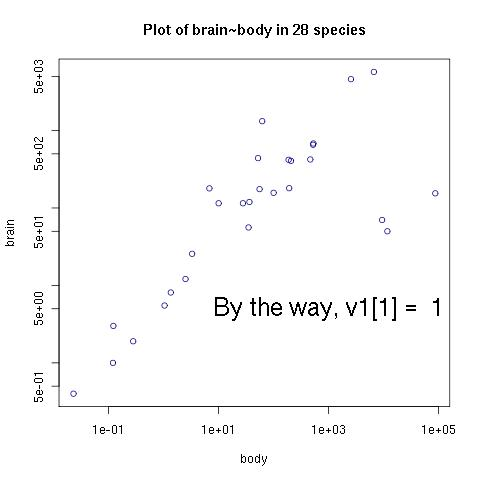
\includegraphics[height=5.5cm]{figs/plot.jpg}  
 \end{center}

\end{frame}

%%%%%%%%%%%%%%%%%%%%%%%%%%%%%%%%%%%%%%%%%%%%%%%%%%%%%%%%%%%%%%%%%%%%%%%

\begin{frame}[fragile]
  
\frametitle{Histogram and KDE}
 \begin{footnotesize}
   \begin{verbatim}
> hist(log10(Animals$body), freq=F)
> lines(density(log10(Animals$body)), col="red", 
lwd=2, lty=2)
   \end{verbatim}
 \end{footnotesize}
\vspace{-1cm}
\begin{figure}
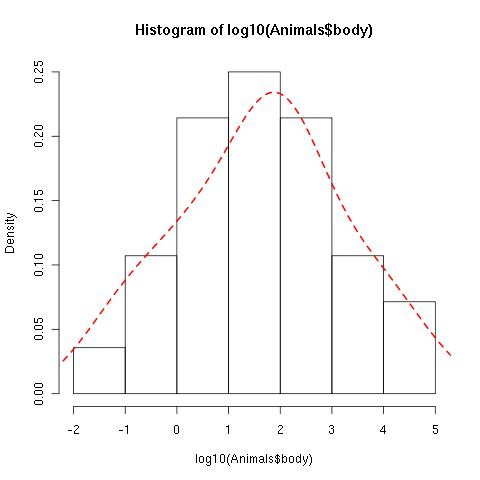
\includegraphics[height=5.5cm]{figs/hist.jpg}
\end{figure}

\end{frame}

%%%%%%%%%%%%%%%%%%%%%%%%%%%%%%%%%%%%%%%%%%%%%%%%%%%%%%%%%%%%%%%%%%%%%%%

\begin{frame}

\frametitle{Box-plot}
   \texttt{> boxplot(Animals, log=``y'')}
\begin{center}
\begin{figure}
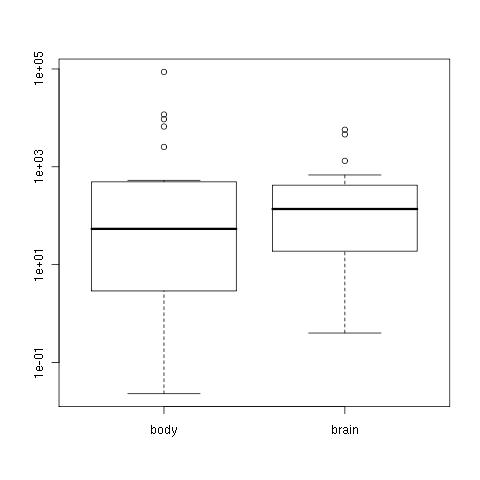
\includegraphics[height=6.0cm]{figs/boxplot.jpg}
\end{figure}
\end{center}

\end{frame}

%%%%%%%%%%%%%%%%%%%%%%%%%%%%%%%%%%%%%%%%%%%%%%%%%%%%%%%%%%%%%%%%%%%%%%%

\begin{frame}[fragile]

 \frametitle{Working with several plots}
 \begin{itemize}
  \item You can create many plots at the same time.
  \item Use \texttt{dev} functions to operate with plots.
 \end{itemize}
 \begin{verbatim}
> dev.new() #Open new plot with next sequential ID
> dev.set(numPlot) #Set numPlot as the active plot
> dev.prev() #What's the previous plot ID?
> dev.next() #What's next plot ID?
> dev.off(numPlot) #Close plot identifed by numPlot
> dev.off() #Close current plot
 \end{verbatim}

\end{frame}

%%%%%%%%%%%%%%%%%%%%%%%%%%%%%%%%%%%%%%%%%%%%%%%%%%%%%%%%%%%%%%%%%%%%%%%

\begin{frame}[fragile]
 \frametitle{Save your plots}
 \begin{itemize}
  \item You can save your plots to files with special devices.\\
 Just call the device before the plotting commands,
 plot your graph and then close the device.
  \item Example
  \begin{verbatim}
> postcript("myFig.eps")
> plot(....)
> # Other plotting commands
> dev.off()
  \end{verbatim}
  \vspace{-0.5cm}
  \item Posible devices
  \begin{verbatim}
> ?Devices #png, jpeg, bmp, tiff, pdf, etc.
  \end{verbatim}
 \end{itemize}
\end{frame}

%%%%%%%%%%%%%%%%%%%%%%%%%%%%%%%%%%%%%%%%%%%%%%%%%%%%%%%%%%%%%%%%%%%%%%%

\section{Working with MySQL DBs}

\begin{frame}[fragile]

\begin{itemize}
 \item You can access MySQL DBs from GNU R.
 \item All you need is: \texttt{> library(RMySQL)}
\end{itemize}
\vspace{-0.5cm}
\begin{verbatim}
 > con <- dbConnect(MySQL(), u="phoenix", p="secret",
 db="evince") #Open DB connection
 > dbListTables(con)
 > dbListFields(con, "table_name")
 > #Execute query, store results in a data frame
 > dbGetQuery(con, "select * from a_table") 
 > dbDisconnect(con) #Close DB connection
 > ?RMySQL # more examples
\end{verbatim}

\end{frame}

%%%%%%%%%%%%%%%%%%%%%%%%%%%%%%%%%%%%%%%%%%%%%%%%%%%%%%%%%%%%%%%%%%%%%%%

\section{Conclusions}

%%%%%%%%%%%%%%%%%%%%%%%%%%%%%%%%%%%%%%%%%%%%%%%%%%%%%%%%%%%%%%%%%%%%%%%

\begin{frame}

\frametitle{Conclusions}
\begin{itemize}
 \item Many libraries ready to faciliate your work.
 \item Save time writing your own scripts.
 \item It is easy to learn new tools reading help files
 \item Working with MySQL (actually with any DB) is
 straightforward
 \item R Helps us producing quality analyses, quality graphs.
\end{itemize}

\end{frame}

%%%%%%%%%%%%%%%%%%%%%%%%%%%%%%%%%%%%%%%%%%%%%%%%%%%%%%%%%%%%%%%%%%%%%%%

\end{document}

